\documentclass[11pt]{article}

\usepackage[margin=1in]{geometry}
\usepackage{amsmath,amssymb,amsthm,mathtools}
\usepackage{booktabs}
\usepackage{enumitem}
\usepackage{float}
\usepackage{graphicx}
\usepackage{microtype}
\usepackage{xcolor}
\usepackage[colorlinks=true,linkcolor=blue!55!black,citecolor=blue!55!black,
  urlcolor=blue!55!black]{hyperref}

\newtheorem{theorem}{Theorem}
\newtheorem{lemma}[theorem]{Lemma}
\newtheorem{corollary}[theorem]{Corollary}
\theoremstyle{definition}
\newtheorem{definition}[theorem]{Definition}
\theoremstyle{remark}
\newtheorem{remark}[theorem]{Remark}

\newcommand{\1}{\mathbf 1}
\newcommand{\R}{\mathbb R}
\newcommand{\Sp}{\mathrm{Sp}}
\newcommand{\SOe}{\mathrm{SO(even)}}
\newcommand{\SOo}{\mathrm{SO(odd)}}
\newcommand{\OO}{\mathrm O}
\newcommand{\ip}[2]{\left\langle #1,#2\right\rangle}
\newcommand{\norm}[1]{\left\lVert #1\right\rVert}

\title{\textbf{An Exact All-Support Matrix Algorithm for the\\
Optimal One-Level Test Function}\\[4pt]
\large Candidate full solution to the coefficient problem in
arXiv:1507.03598 and arXiv:1708.01588}
\author{Automated mathematics discovery run \texttt{fa\_banach\_001}\\
Agent \texttt{agent\_lane\_08} (GPT5.6)}
\date{July 23, 2026}

\begin{document}
\maketitle

\begin{center}
\fbox{\parbox{0.91\textwidth}{
\textbf{Status.} Candidate full solution, likely valid, pending expert
review. The result gives a square, nonsingular matrix system for every
positive support parameter and every classical compact symmetry type. It
also proves the continuity and piecewise real-analyticity conjectured in
arXiv:1708.01588, Conjecture 12.1.
}}
\end{center}

\begin{abstract}
Freeman and Miller reduced optimal one-level test functions to a Fredholm
equation and asked for an all-support algorithm that selects the correct
coefficients from the delay-differential solution family. Freeman later
obtained an all-support finite-dimensional family but left the coefficient
optimization open. We give a direct finite algorithm. After translating the
support interval to $[0,L]$, split it at the points of
$(\mathbb Z\cup(L+\mathbb Z))\cap[0,L]$. Translation by one permutes the
resulting cells in two chains. On each chain the differentiated Fredholm
equation is a constant-coefficient ODE with a skew tridiagonal matrix.
Matrix exponentials, continuity at cell boundaries, and one undifferentiated
normalization equation form a square linear system. A strict operator-norm
bound proves that this system is nonsingular for every $L>0$. The system
therefore computes the unique optimal factor and test function for all
support restrictions. Analytic dependence of the finite system away from
integer $L$, together with Hilbert--Schmidt resolvent continuity at integer
$L$, proves the later regularity conjecture.
\end{abstract}

\section{Source question and later sharpened problem}

The source is Jesse Freeman and Steven J. Miller,
\emph{Determining Optimal Test Functions for Bounding the Average Rank in
Families of $L$-Functions}, arXiv:1507.03598 \cite{FM2015}. In Section 6,
page 16 of the arXiv PDF, they conjecture that their method provides
solutions for all positive $\sigma$. They isolate two steps: solving the
delay-differential system and selecting the coefficients that give the
optimal factor $g$. They note that even an all-support algorithm for the
first step would reduce the infinite-dimensional problem to finite
dimensions.

\begin{figure}[H]
\centering

\includegraphics[width=\textwidth]{figures/open_problem_crop.png}
\caption{The all-support conjecture and algorithmic problem in
arXiv:1507.03598, Section 6, page 16. This is a direct crop from
\texttt{source\_paper.pdf}.}
\end{figure}

Freeman's later paper \emph{Fredholm Theory and Optimal Test Functions for
Detecting Central Point Vanishing Over Families of $L$-functions},
arXiv:1708.01588 \cite{Freeman2017}, proves that the solution family is
finite-dimensional for every $\sigma$. Corollary 9.9 computes its dimension.
Section 12.1, page 62 (PDF page 63), says that the remaining finite
optimization had only been solved for
$1<\sigma<3/2$ and $3/2<\sigma<2$, asks for a general solution, and states:
\[
\text{``$\mathfrak I_G(\sigma)$ is continuous in $\sigma$ and is
real-analytic except at integers and half-integers.''}
\]

\begin{figure}[H]
\centering
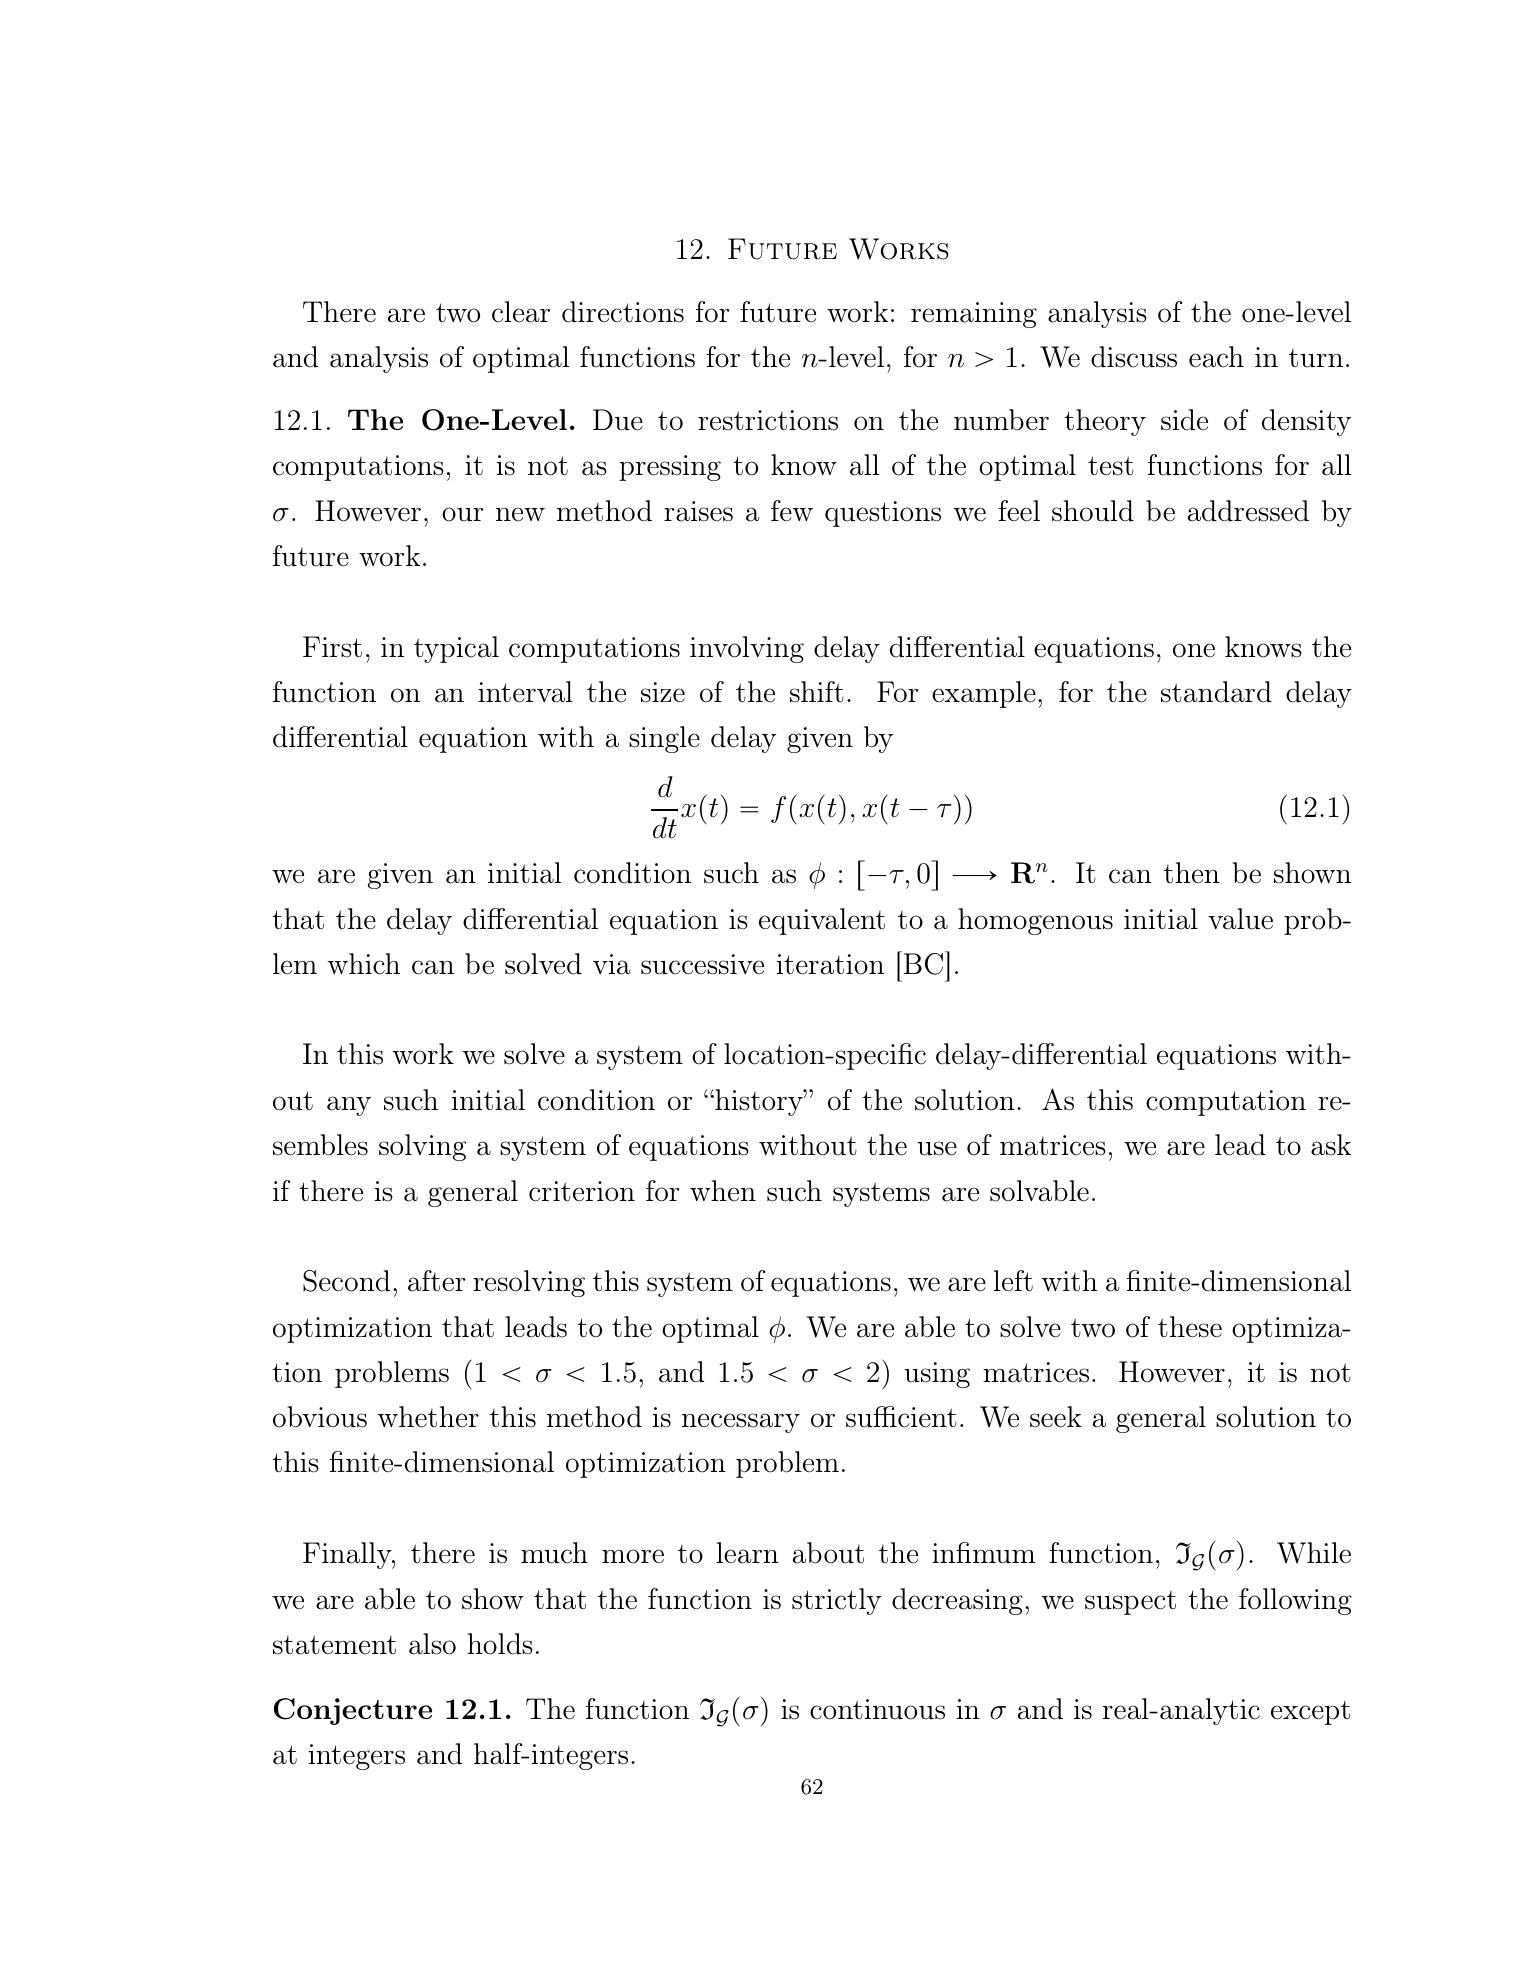
\includegraphics[height=0.82\textheight]{figures/supporting_open_problem_crop.png}
\caption{The open coefficient problem and Conjecture 12.1 in
arXiv:1708.01588, Section 12.1, printed page 62. This is a direct crop from
\texttt{supporting\_paper\_1708.01588.pdf}.}
\end{figure}

\section{Normalized Fredholm problem}

Put $L=2\sigma$ and translate $[-\sigma,\sigma]$ to $[0,L]$. Define the
compact self-adjoint operator
\[
 (T_Lf)(t)=\int_0^L \1_{\{|t-s|\leq 1\}}f(s)\,ds
 \qquad (0\leq t\leq L).
\]
For $\beta\in\{1/2,-1/2\}$ set
\[
 A_{\beta,L}=I+\beta T_L.
\]
The normalized optimality equations for $\SOe$ and $\Sp$ are respectively
\[
 A_{1/2,L}q_+=\1,
 \qquad
 A_{-1/2,L}q_-=\1.                                      \tag{2.1}
\]
The other two symmetry types are rank-one consequences. If
$P_Lf=\ip{f}{\1}\1$ and $Q_-=\int_0^Lq_-(t)\,dt$, then
\[
\begin{aligned}
 g_{\SOe}&=q_+,&
 g_{\Sp}&=q_-,\\
 g_{\SOo}&=\frac{q_-}{1+Q_-},&
 g_{\OO}&=\frac{\1}{1+L/2}.
\end{aligned}                                             \tag{2.2}
\]
Indeed, the $\SOo$ operator is $A_{-1/2,L}+P_L$, while the $\OO$
operator is $I+\tfrac12P_L$.

\begin{lemma}[Strict norm bound]\label{lem:norm}
For every finite $L>0$,
\[
 \norm{T_L}_{L^2(0,L)\to L^2(0,L)}<2.
\]
Consequently $A_{1/2,L}$ and $A_{-1/2,L}$ are positive and invertible.
\end{lemma}

\begin{proof}
The kernel of $T_L$ belongs to $L^2([0,L]^2)$, so $T_L$ is compact.
Extend $f\in L^2(0,L)$ by zero to $\widetilde f\in L^2(\R)$. The extension
of $T_Lf$ by zero is the compression to $[0,L]$ of
$\1_{[-1,1]}*\widetilde f$. By Plancherel,
\[
 \norm{\1_{[-1,1]}*\widetilde f}_2^2
 =\int_{\R}|m(\xi)|^2|\widehat{\widetilde f}(\xi)|^2\,d\xi,
\]
where the convolution multiplier $m$ satisfies $|m(\xi)|\leq2$, with
equality only at the single frequency $\xi=0$. Thus every nonzero $f$
satisfies
\[
 \norm{T_Lf}_2
 \leq\norm{\1_{[-1,1]}*\widetilde f}_2
 <2\norm f_2.
\]
If $\norm{T_L}=2$, compactness would give a unit vector at which the norm is
attained, contradicting the strict inequality. Hence $\norm{T_L}<2$.
Since $T_L$ is self-adjoint, the spectra of $I\pm T_L/2$ lie in
$(0,2)$.
\end{proof}

\section{The exact finite system}

For $m\geq1$, let $A_m(\beta)$ be the $m$-by-$m$ skew tridiagonal matrix
\[
 (A_m)_{j,j+1}=-\beta,\qquad
 (A_m)_{j+1,j}=\beta
 \quad (0\leq j<m-1),
\]
with all other entries zero. Put
\[
 E_m(t)=e^{tA_m(\beta)},\qquad
 J_m(t)=\int_0^t e^{sA_m(\beta)}\,ds.                    \tag{3.1}
\]
The formula for $J_m$ is valid even when $A_m$ is singular; it can be
evaluated by one block-matrix exponential.

\subsection{Noninteger length}

Write $L=N+r$, where $N=\lfloor L\rfloor$ and $0<r<1$. Split $[0,L]$ into
\[
 R_k=[k,k+r]\quad(0\leq k\leq N),\qquad
 S_k=[k+r,k+1]\quad(0\leq k<N).                          \tag{3.2}
\]
Let $u\in\R^{N+1}$ and $v\in\R^N$. For $N\geq1$, determine them from the
$2N+1$ equations
\begin{align}
 (E_{N+1}(r)u)_k&=v_k
        &&(0\leq k<N),                                   \tag{3.3}\\
 (E_N(1-r)v)_k&=u_{k+1}
        &&(0\leq k<N),                                   \tag{3.4}\\
 u_0+\beta\big((J_{N+1}(r)u)_0+(J_N(1-r)v)_0\big)&=1.
                                                               \tag{3.5}
\end{align}
Then reconstruct $q=q_{\beta,L}$ by
\begin{align}
 q(k+s)&=(E_{N+1}(s)u)_k
       &&(0\leq k\leq N,\ 0\leq s\leq r),                \tag{3.6}\\
 q(k+r+s)&=(E_N(s)v)_k
       &&(0\leq k<N,\ 0\leq s\leq1-r).                   \tag{3.7}
\end{align}
When $0<L<1$, there is only one cell and the formula reduces to
\[
 q(t)=\frac{1}{1+\beta L}.                               \tag{3.8}
\]

\subsection{Integer length}

If $L=N\in\mathbb N$, determine $u\in\R^N$ from the $N$ equations
\begin{align}
 (E_N(1)u)_k&=u_{k+1}
       &&(0\leq k<N-1),                                  \tag{3.9}\\
 u_0+\beta(J_N(1)u)_0&=1,                                \tag{3.10}
\end{align}
and set
\[
 q(k+s)=(E_N(s)u)_k
 \quad(0\leq k<N,\ 0\leq s\leq1).                        \tag{3.11}
\]

\begin{theorem}[All-support coefficient algorithm]\label{thm:algorithm}
For every $L>0$ and $\beta\in\{1/2,-1/2\}$, the appropriate system
\emph{(3.3)--(3.5)} or \emph{(3.9)--(3.10)} is square and nonsingular. Its
reconstruction is the unique solution of
\[
 (I+\beta T_L)q=\1.                                      \tag{3.12}
\]
Thus \emph{(2.2)} computes all four normalized optimal factors for every
positive support parameter.
\end{theorem}

\begin{proof}
We first prove exactness. Away from the breakpoints
$(\mathbb Z\cup(L+\mathbb Z))\cap[0,L]$, differentiation of (3.12) gives
\[
 q'(t)=-\beta\,\1_{\{t+1<L\}}q(t+1)
        +\beta\,\1_{\{t-1>0\}}q(t-1).                    \tag{3.13}
\]
Translation by one preserves each chain of cells in (3.2). If the
restrictions of $q$ to a chain are assembled into a vector $y(s)$ in
left-to-right order, (3.13) is exactly
\[
 y'(s)=A_m(\beta)y(s).                                   \tag{3.14}
\]
Equations (3.3) and (3.4), or (3.9), are precisely the continuity
conditions at consecutive cell boundaries.

For a reconstructed continuous function define
\[
 F(t)=q(t)+\beta\int_0^L\1_{\{|t-s|\leq1\}}q(s)\,ds.
\]
Equation (3.14) gives $F'(t)=0$ on every open cell. Since $F$ is continuous,
it is one constant on all of $[0,L]$. Equations (3.5) and (3.10) are exactly
$F(0)=1$, so the reconstruction solves (3.12).

Conversely, an $L^2$ solution of (3.12) is continuous because the moving
window integral is continuous. On each open cell it is differentiable and
satisfies (3.13), hence (3.14), and therefore yields endpoint data satisfying
the displayed finite system.

It remains to prove nonsingularity. A vector in the kernel of the homogeneous
finite system would reconstruct a solution of
$(I+\beta T_L)q=0$. Lemma \ref{lem:norm} forces $q=0$, and the endpoint
vector is then zero. The square coefficient matrix has trivial kernel and is
nonsingular. Existence and uniqueness follow.
\end{proof}

\begin{remark}[Dimension check]
Off integer $L$, the system has $2\lfloor L\rfloor+1$ unknowns. At integer
$L$ it has $L$ unknowns. Since $L=2\sigma$, these become
\[
\begin{array}{c|c}
\text{support range}&\text{dimension}\\ \hline
k<\sigma<k+\tfrac12&4k+1\\
k+\tfrac12<\sigma<k+1&4k+3\\
\sigma=k&2k\\
\sigma=k+\tfrac12&2k+1,
\end{array}
\]
which agrees exactly with Freeman's Corollary 9.9 \cite{Freeman2017}. The
new equations select the unique coefficient vector in that family.
\end{remark}

\section{Proof intuition}

The source difficulty is that differentiating the Fredholm equation loses
one scalar constant and appears to produce a delay equation without an
initial history. The breakpoints remove both obstacles. They are exactly the
places at which either $t+1$ or $t-1$ enters or leaves the support. Between
them, translation by one never changes combinatorial type, so all translated
pieces of $q$ evolve together by one constant skew tridiagonal matrix.

Matrix exponentials therefore solve the delay system without prescribing an
arbitrary history. Continuity glues the cell solutions, while a single
undifferentiated equation at $t=0$ restores the scalar constant lost under
differentiation. Finally, Fredholm invertibility turns the resulting square
system from a candidate construction into a guaranteed algorithm: a
singular coefficient matrix would manufacture a forbidden homogeneous
Fredholm solution.

\section{Optimality and the test function}

The source papers identify the admissible Fourier transforms as
\[
 \widehat\phi=g*\check g,\qquad
 \check g(x)=\overline{g(-x)},\qquad
 \operatorname{supp}g\subset[-\sigma,\sigma].
                                                               \tag{5.1}
\]
For completeness, optimality of the factor produced above follows directly
from positivity. Let $B_G$ be the corresponding positive operator:
\[
\begin{aligned}
B_{\SOe}&=I+\tfrac12T_L,&
B_{\Sp}&=I-\tfrac12T_L,\\
B_{\SOo}&=I-\tfrac12T_L+P_L,&
B_{\OO}&=I+\tfrac12P_L.
\end{aligned}
\]
If $g_G=B_G^{-1}\1$, then for every nonzero admissible factor $h$,
Cauchy--Schwarz in the $B_G$ inner product gives
\[
 |\ip{h}{\1}|^2
 =|\ip{B_G^{1/2}h}{B_G^{-1/2}\1}|^2
 \leq \ip{B_Gh}{h}\,\ip{g_G}{\1}.                        \tag{5.2}
\]
Hence
\[
 \frac{\ip{B_Gh}{h}}{|\ip{h}{\1}|^2}
 \geq\frac{1}{\int_0^L g_G(t)\,dt},                      \tag{5.3}
\]
with equality exactly for scalar multiples of $g_G$. The normalization
$B_Gg_G=\1$ fixes the scalar. Translating $g_G$ back to
$[-\sigma,\sigma]$ and applying (5.1) yields the optimal test function
\[
 \phi_G=\left|\mathcal F^{-1}g_G\right|^2.                \tag{5.4}
\]
The optimal infimum is
\[
 \mathfrak I_G(\sigma)
 =\frac{1}{\int_0^L g_G(t)\,dt}.                         \tag{5.5}
\]
In particular, if $Q_\pm=\int_0^Lq_\pm$, then
\[
\begin{aligned}
\mathfrak I_{\SOe}(\sigma)&=Q_+^{-1},&
\mathfrak I_{\Sp}(\sigma)&=Q_-^{-1},\\
\mathfrak I_{\SOo}(\sigma)&=1+Q_-^{-1},&
\mathfrak I_{\OO}(\sigma)&=\frac1L+\frac12.
\end{aligned}                                             \tag{5.6}
\]

\section{Full regularity classification}

\begin{theorem}[Conjecture 12.1]\label{thm:regularity}
For each $G\in\{\SOe,\Sp,\SOo,\OO\}$, the function
$\mathfrak I_G:(0,\infty)\to\R$ is continuous. It is real-analytic on every
component of
\[
 (0,\infty)\setminus\tfrac12\mathbb Z.
\]
Thus Freeman's Conjecture 12.1 holds. For $G=\OO$, the function is in fact
real-analytic on all of $(0,\infty)$.
\end{theorem}

\begin{proof}
Fix an integer $N\geq0$. For $L=N+r$ with $0<r<1$, every entry of the system
matrix in (3.3)--(3.5) is real-analytic in $r$: its entries are formed from
$e^{rA}$, $e^{(1-r)A}$, and their integrals. The determinant never vanishes
by Theorem \ref{thm:algorithm}. Cramer's rule, or analytic matrix inversion,
shows that $u$, $v$, and
\[
 Q_{\beta,L}
 =\mathbf 1^\mathsf TJ_{N+1}(r)u
  +\mathbf 1^\mathsf TJ_N(1-r)v                          \tag{6.1}
\]
are real-analytic in $r$ (with the evident one-cell formula when $N=0$).
The formulas (2.2) and (5.6) preserve real-analyticity. Positivity guarantees
that every denominator is nonzero.

It remains to cross integer values of $L$. Work on the fixed space
$L^2(\R)$ and extend the interval operator by zero. Its kernel is
\[
 k_L(x,y)=\1_{[0,L]}(x)\1_{[0,L]}(y)\1_{\{|x-y|\leq1\}}.
                                                               \tag{6.2}
\]
As $L'\to L$, $k_{L'}\to k_L$ in $L^2(\R^2)$, so the corresponding
operators converge in Hilbert--Schmidt, hence operator, norm. Also
$\1_{[0,L']}\to\1_{[0,L]}$ in $L^2(\R)$. Since
$I\pm T_L/2$ is invertible, the resolvent identity gives local
operator-norm continuity of its inverse. Therefore the zero extensions
\[
 q_{\pm,L}=(I\pm T_L/2)^{-1}\1_{[0,L]}
\]
vary continuously in $L^2(\R)$. Their integrals are the inner products
$\ip{q_{\pm,L}}{\1_{[0,L]}}$ and are continuous. Equations (2.2) and (5.6)
then prove continuity for every symmetry type. Finally, $L=2\sigma$, so
integer breakpoints in $L$ are precisely the integers and half-integers in
$\sigma$.
\end{proof}

\section{Computational verification}

The included script \texttt{code/verify\_algorithm.py} independently builds
the breakpoint orbits, constructs the square system through matrix
exponentials, and evaluates the Fredholm residual on a 401-point grid.
It tests both signs of $\beta$ and the $\SOo$ rank-one rescaling.

\begin{center}
\begin{tabular}{@{}lll@{}}
\toprule
Tested $L$ values & Main maximum residual & Additional check\\
\midrule
$0.4,1,1.4,2,2.4,3,3.7,5.25,8.1$
& $<4.3\cdot10^{-14}$ & both $\beta=\pm1/2$\\
$1\pm10^{-6},2\pm10^{-6},3\pm10^{-6}$
& $<2\cdot10^{-8}$ & one-sided integral continuity\\
\bottomrule
\end{tabular}
\end{center}

Run from the repository root with
\begin{verbatim}
conda run --no-capture-output -n sandbox python \
  runs/fa_banach_001/solutions/full/\
1507.03598_all_support_optimal_test_function_algorithm/code/verify_algorithm.py
\end{verbatim}
The numerical calculation is not used as proof; it pressure-tests signs,
cell indexing, continuity equations, normalization, and the rank-one
formula.

\section{Novelty check, scope, and review priorities}

\paragraph{Bounded search.}
On July 23, 2026, the local registry, solution, attempt, and proof-gap
indexes were searched for arXiv ids 1507.03598 and 1708.01588 and for the
core phrases ``optimal test function'', ``finite-dimensional
optimization'', and ``real-analytic except at integers and half-integers''.
Bounded arXiv searches used the two arXiv ids, the authors Freeman and
Miller, ``matrix exponential'', ``all support'', ``coefficient'', and
``Conjecture 12.1''. The search found Freeman's 2017 all-support
finite-dimensional reduction \cite{Freeman2017} and the later restricted
two-level extension arXiv:2011.10140 \cite{BCDMZ2020}. No paper was found
that gives the square all-support coefficient system above or states a
proof of Conjecture 12.1. This supports, but cannot guarantee, novelty.

\paragraph{Scope.}
The theorem solves the one-level compact-group optimization problem with
the indicator kernels used in the source papers. It does not verify a
number-theoretic density theorem at new support, incorporate lower-order
terms, or solve unrestricted higher-level density optimization.

\paragraph{Human-review priorities.}
The most valuable checks are:
\begin{enumerate}[leftmargin=2em]
\item verify the translation from the source interval and kernels to
      (2.1)--(2.2);
\item check the two cell-chain endpoint conventions in (3.3)--(3.7);
\item confirm that the source admissibility/factorization theorem permits
      the variational conclusion (5.4) at every positive support;
\item search citations to arXiv:1708.01588 for a later unpublished or
      differently phrased solution.
\end{enumerate}

\begin{thebibliography}{9}

\bibitem{FM2015}
Jesse Freeman and Steven J. Miller,
\emph{Determining Optimal Test Functions for Bounding the Average Rank in
Families of $L$-Functions},
arXiv:1507.03598, 2015.
\url{https://arxiv.org/abs/1507.03598}.

\bibitem{Freeman2017}
Jesse Freeman,
\emph{Fredholm Theory and Optimal Test Functions for Detecting Central Point
Vanishing Over Families of $L$-functions},
arXiv:1708.01588, 2017.
\url{https://arxiv.org/abs/1708.01588}.

\bibitem{BCDMZ2020}
Elzbieta Boldyriew, Fangu Chen, Charles Devlin VI, Steven J. Miller, and
Jason Zhao,
\emph{Determining Optimal Test Functions for $2$-Level Densities},
arXiv:2011.10140, 2020.
\url{https://arxiv.org/abs/2011.10140}.

\end{thebibliography}

\end{document}
